\documentclass[10pt,a4paper]{article}
\usepackage[margin=22mm]{geometry}
\usepackage[T1]{fontenc}
\usepackage[utf8]{inputenc}
\usepackage{lmodern,microtype,graphicx,booktabs,longtable,array,amsmath,caption,pdflscape,placeins}
\usepackage[numbers,sort&compress]{natbib}
\usepackage[hidelinks]{hyperref}
\graphicspath{{../figures/main/}{../figures/supplementary/}}
\setlength{\emergencystretch}{2em}
\newcommand{\ExtensionModel}{random forest}
\newcommand{\ExtensionFOne}{0.821}
\newcommand{\ExtensionCV}{0.695}
\newcommand{\ExtensionLow}{0.691}
\newcommand{\ExtensionHigh}{0.835}
\newcommand{\ExtensionAgreement}{0.813}

\begin{document}
\renewcommand{\thesection}{S\arabic{section}}
\renewcommand{\thetable}{S\arabic{table}}
\renewcommand{\thefigure}{S\arabic{figure}}
\begin{center}\Large\bfseries Supplementary Information\end{center}
\begin{center}Sensitivity-aware inspection prioritisation for archaeological landscapes: a reproducible Taxila observatory\end{center}
\section{Supporting methods and complete experimental results}
The main article presents the multitemporal maps, score baselines, ablations, support and joint-uncertainty experiments, and the climate comparison. This supplement provides full component inventories, numerical tables, configurations and secondary diagnostics. Spatial simulations and land-cover agreement have the distinct scopes specified in the main methods. The public archive additionally contains a weakly supervised land-cover classification benchmark carried out during development. It addresses a different question from the one posed here, supports no claim in this article, and is retained in the archive for completeness only.

\section{Component inventory and analytical support}
Saraikala is preserved without invented geometry. Coordinates are inventory points, not property polygons. The same 17 mapped components are compared at all three radii.
\begingroup
\scriptsize
\setlength{\tabcolsep}{3pt}
\begin{longtable}{p{0.10\textwidth}p{0.30\textwidth}p{0.24\textwidth}rrp{0.08\textwidth}}
\caption{Complete Taxila component inventory and analytical geometry status.}\label{tab:s-component-inventory}\\
\toprule
ID & Component & Coordinate status & Longitude & Latitude & Included \\
\midrule
\endfirsthead
\caption[]{Complete Taxila component inventory and analytical geometry status. (continued)}\\
\toprule
ID & Component & Coordinate status & Longitude & Latitude & Included \\
\midrule
\endhead
\midrule
\multicolumn{6}{r}{Continued on next page}\\
\endfoot
\bottomrule
\endlastfoot
139-001 & Khanpur Cave & official\_web\_point & 72.909294 & 33.799200 & Yes \\
139-002 & Saraikala, prehistoric mound & official\_id\_geometry\_missing &  &  & No \\
139-003 & Bhir Mound & official\_web\_point & 72.819331 & 33.743944 & Yes \\
139-004 & Sirkap (fortified city) & official\_web\_point & 72.829878 & 33.753403 & Yes \\
139-005 & Sirsukh (fortified ruined city) & official\_web\_point & 72.849739 & 33.772256 & Yes \\
139-006 & Dharmarajika stupa and monastery & official\_web\_point & 72.842667 & 33.744669 & Yes \\
139-007 & Khader Mohra (Akhuri) & official\_web\_point & 72.860722 & 33.760806 & Yes \\
139-008 & Kalawan group of buildings & official\_web\_point & 72.839753 & 33.746292 & Yes \\
139-009 & Giri complex of monuments & official\_web\_point & 72.883325 & 33.729089 & Yes \\
139-010 & Kunala stupa and monastery & official\_web\_point & 72.831444 & 33.750553 & Yes \\
139-011 & Jandial complex & official\_web\_point & 72.828914 & 33.764456 & Yes \\
139-012 & Lalchak and Badalpur Buddhist stuppa & official\_web\_point & 72.868019 & 33.781803 & Yes \\
139-013 & Mohra Moradu stupa and monastery & official\_web\_point & 72.861053 & 33.761097 & Yes \\
139-014 & Pippala stupa and monastery & official\_web\_point & 72.866686 & 33.765922 & Yes \\
139-015 & Jaulian stupa and monastery & official\_web\_point & 72.875311 & 33.765042 & Yes \\
139-016 & Lalchak mounds & official\_web\_point & 72.849469 & 33.774450 & Yes \\
139-017 & Buddhist remains around Bhallar stupa & official\_web\_point & 72.825358 & 33.813497 & Yes \\
139-018 & Giri Mosque and tombs & official\_web\_point & 72.880522 & 33.727769 & Yes \\
\end{longtable}
\noindent\textit{Note:} Coordinates are WGS 84 point locations transcribed from the official component map. Saraikala remains in the inventory but is excluded from coordinate-dependent analysis. Analytical circles are not official property polygons or legal buffers.
\endgroup

\section{Annual climate analysis}
The procedure resamples detrended residual blocks. A trend-restored ensemble supplies confidence intervals; a constant-baseline ensemble supplies null slopes. The 12 annual metrics form the multiplicity family. Heavy precipitation counts days exceeding the 1991--2020 wet-day 95th percentile (wet days have at least 1 mm rain); hot days exceed the baseline maximum-temperature 95th percentile. Heatwave duration is the longest run above that temperature threshold, without a separate minimum-duration criterion. Dry-spell duration counts consecutive days below 1 mm. Rx1day and Rx5day are the largest one-day and rolling five-day precipitation totals.

\begingroup\scriptsize\setlength{\tabcolsep}{3pt}\begin{longtable}{p{.35\linewidth}rrrrr}
\caption{Annual residual-block trends; 2,000 draws and five-year blocks.} \\
\toprule
Metric & Slope/year & CI low & CI high & p & Annual q \\
\midrule
\endfirsthead
\caption[]{Annual residual-block trends; 2,000 draws and five-year blocks.} \\
\toprule
Metric & Slope/year & CI low & CI high & p & Annual q \\
\midrule
\endhead
\midrule
\multicolumn{6}{r}{Continued on next page} \\
\midrule
\endfoot
\bottomrule
\endlastfoot
precipitation\_sum\_mm & -10.3037 & -17.9150 & -2.6679 & 0.0090 & 0.0270 \\
rx1day\_mm & -0.6233 & -1.5426 & 0.4034 & 0.1549 & 0.2324 \\
rx5day\_mm & -1.7354 & -3.3891 & -0.2019 & 0.0395 & 0.0948 \\
heavy\_precipitation\_days & -0.1429 & -0.2266 & -0.0582 & 0.0015 & 0.0180 \\
consecutive\_dry\_days & 0.1667 & -0.1417 & 0.4322 & 0.2029 & 0.2597 \\
temperature\_mean\_c & 0.0418 & 0.0099 & 0.0731 & 0.0065 & 0.0260 \\
annual\_or\_period\_max\_tmax\_c & 0.0333 & -0.0079 & 0.0778 & 0.1204 & 0.2065 \\
hot\_days & 0.1818 & -0.1728 & 0.5227 & 0.3063 & 0.3342 \\
heatwave\_max\_days & 0.0323 & -0.0449 & 0.1144 & 0.3493 & 0.3493 \\
relative\_humidity\_mean\_percent & -0.1311 & -0.2852 & 0.0255 & 0.1124 & 0.2065 \\
soil\_moisture\_mean\_m3m3 & -0.0013 & -0.0022 & -0.0003 & 0.0065 & 0.0260 \\
et0\_sum\_mm & 2.2850 & -1.2405 & 5.5941 & 0.2164 & 0.2597 \\
\end{longtable}
\endgroup
Precipitation and evapotranspiration slopes are in mm year$^{-1}$, temperature slopes in $^\circ$C year$^{-1}$, humidity in percentage points year$^{-1}$, soil moisture in m$^3$ m$^{-3}$ year$^{-1}$ and event counts in days year$^{-1}$. Effective-sample-size diagnostics use detrended lag-one correlation and are bounded by the observed record length; they do not replace the bootstrap.
\begin{figure}[tbp]\centering
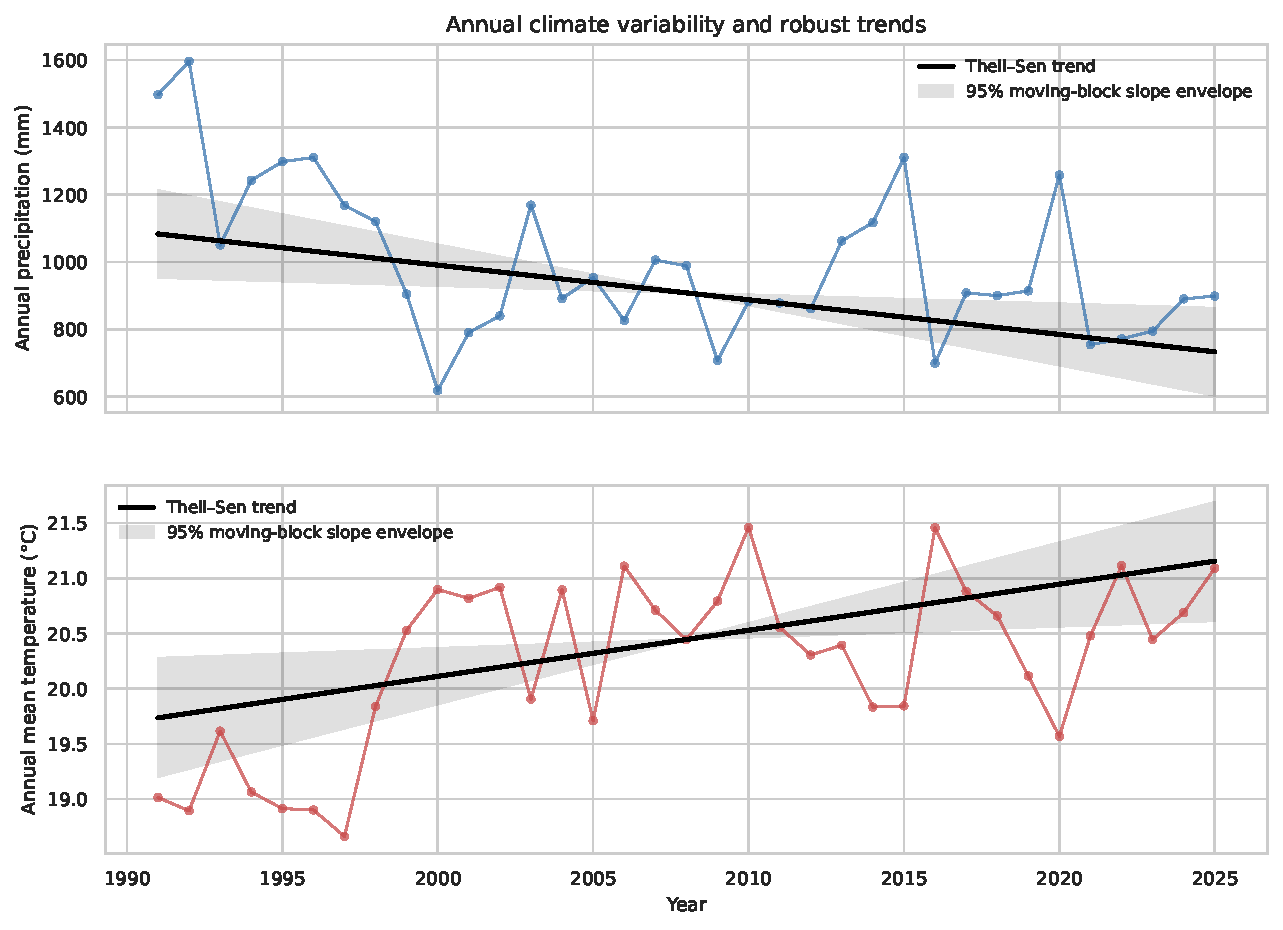
\includegraphics[width=\textwidth]{figure_s01_annual_climate_trends.pdf}
\caption{Annual climate series and robust trend fits for the regional four-cell average, 1991--2025. Intervals are residual-block replicates; inference is conditional on the weather product.}\label{fig:s-trends}
\end{figure}

\begin{figure}[tbp]\centering
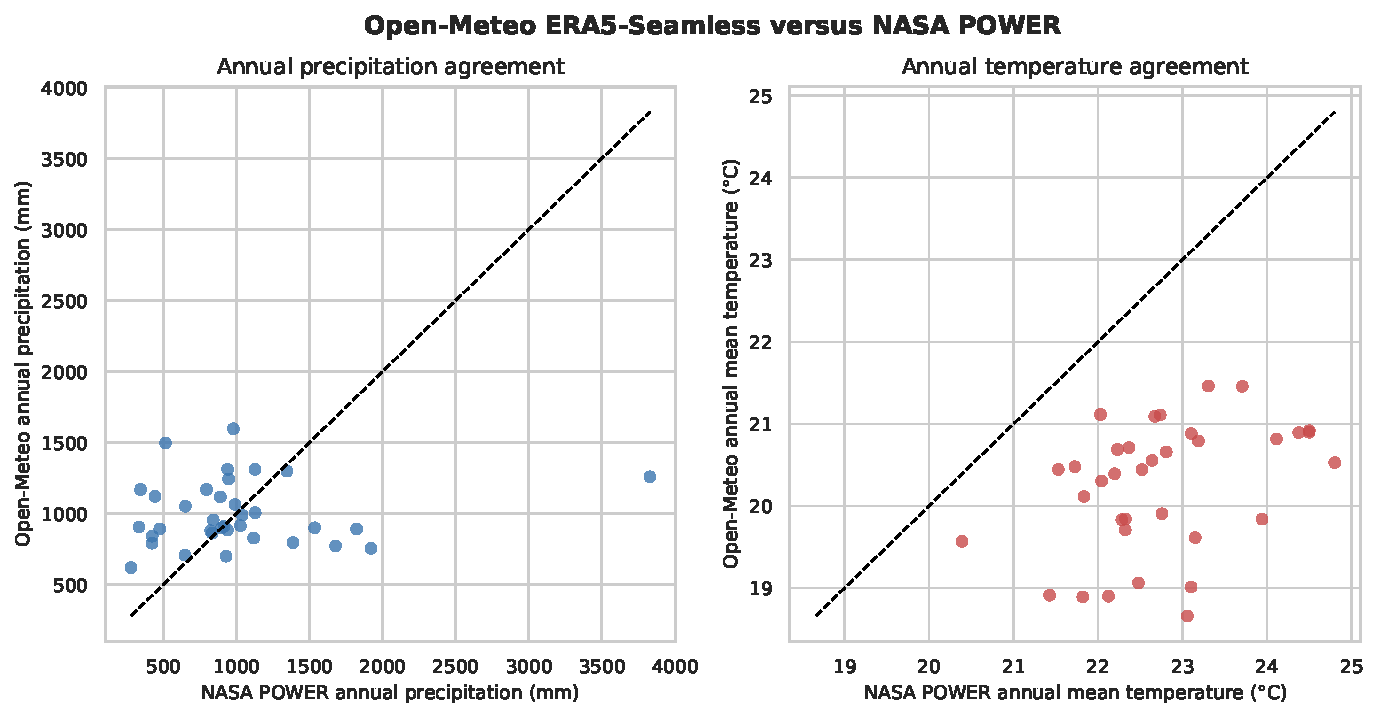
\includegraphics[width=\textwidth]{figure_s02_weather_product_comparison.pdf}
\caption{Matched annual precipitation and temperature in the two gridded weather products. Dashed lines indicate equality. Product disagreement constrains environmental interpretation in the absence of station validation; this figure was carried in the main article of earlier manuscript generations.}\label{fig:s-weather}
\end{figure}
\section{Ranks and uncertainty scope}
The following tables report component scores and two complementary sensitivity designs. The weight experiment perturbs the integrated domain architecture; the spatial experiment resamples 150 m spectral blocks with terrain fixed. They must not be described as the same probability distribution.

\begin{longtable}{lrrrr}
\caption{Component scores and scale-dependent ranks.} \\
\toprule
Component & Rank 250 m & Rank 500 m & Rank 1,000 m & Score 500 m \\
\midrule
\endfirsthead
\caption[]{Component scores and scale-dependent ranks.} \\
\toprule
Component & Rank 250 m & Rank 500 m & Rank 1,000 m & Score 500 m \\
\midrule
\endhead
\midrule
\multicolumn{5}{r}{Continued on next page} \\
\midrule
\endfoot
\bottomrule
\endlastfoot
139-001 & 15.0000 & 14.0000 & 11.0000 & 0.4309 \\
139-003 & 14.0000 & 17.0000 & 17.0000 & 0.3397 \\
139-004 & 10.0000 & 12.0000 & 15.0000 & 0.4799 \\
139-005 & 8.0000 & 9.0000 & 10.0000 & 0.5015 \\
139-006 & 3.0000 & 5.0000 & 6.0000 & 0.5363 \\
139-007 & 7.0000 & 6.0000 & 3.0000 & 0.5353 \\
139-008 & 12.0000 & 7.0000 & 9.0000 & 0.5191 \\
139-009 & 4.0000 & 1.0000 & 2.0000 & 0.5912 \\
139-010 & 5.0000 & 10.5000 & 13.0000 & 0.5010 \\
139-011 & 16.0000 & 16.0000 & 16.0000 & 0.3485 \\
139-012 & 17.0000 & 15.0000 & 12.0000 & 0.3922 \\
139-013 & 11.0000 & 4.0000 & 5.0000 & 0.5392 \\
139-014 & 6.0000 & 10.5000 & 8.0000 & 0.5010 \\
139-015 & 2.0000 & 3.0000 & 1.0000 & 0.5676 \\
139-016 & 13.0000 & 13.0000 & 14.0000 & 0.4461 \\
139-017 & 9.0000 & 8.0000 & 7.0000 & 0.5172 \\
139-018 & 1.0000 & 2.0000 & 4.0000 & 0.5725 \\
\end{longtable}

\begin{longtable}{lrrrr}
\caption{Spatial-block rank uncertainty; terrain held fixed.} \\
\toprule
Component & Median rank & Low & High & Top-3 frequency \\
\midrule
\endfirsthead
\caption[]{Spatial-block rank uncertainty; terrain held fixed.} \\
\toprule
Component & Median rank & Low & High & Top-3 frequency \\
\midrule
\endhead
\midrule
\multicolumn{5}{r}{Continued on next page} \\
\midrule
\endfoot
\bottomrule
\endlastfoot
139-017 & 1.0000 & 1.0000 & 5.0000 & 0.9110 \\
139-009 & 2.0000 & 1.0000 & 3.0000 & 0.9855 \\
139-018 & 3.0000 & 1.9750 & 5.0000 & 0.6150 \\
139-015 & 4.0000 & 2.0000 & 8.5000 & 0.2940 \\
139-006 & 6.0000 & 3.0000 & 11.0000 & 0.0385 \\
139-013 & 8.0000 & 3.0000 & 15.0000 & 0.0510 \\
139-014 & 8.0000 & 3.5000 & 12.0000 & 0.0245 \\
139-010 & 8.0000 & 4.5000 & 12.0000 & 0.0055 \\
139-007 & 9.0000 & 3.0000 & 15.0000 & 0.0465 \\
139-008 & 9.0000 & 4.5000 & 14.0000 & 0.0040 \\
139-005 & 9.0000 & 5.5000 & 13.0000 & 0.0005 \\
139-004 & 10.0000 & 6.0000 & 13.0000 & 0.0010 \\
139-016 & 14.0000 & 11.0000 & 16.0000 & 0.0000 \\
139-011 & 14.0000 & 12.0000 & 16.0000 & 0.0000 \\
139-001 & 14.0000 & 8.5000 & 16.0000 & 0.0005 \\
139-003 & 16.0000 & 13.0000 & 16.0000 & 0.0000 \\
139-012 & 17.0000 & 16.0000 & 17.0000 & 0.0000 \\
\end{longtable}

\begin{longtable}{lrrrr}
\caption{50,000-draw integrated-domain weight sensitivity.} \\
\toprule
Component & Median rank & Low & High & Top-3 frequency \\
\midrule
\endfirsthead
\caption[]{50,000-draw integrated-domain weight sensitivity.} \\
\toprule
Component & Median rank & Low & High & Top-3 frequency \\
\midrule
\endhead
\midrule
\multicolumn{5}{r}{Continued on next page} \\
\midrule
\endfoot
\bottomrule
\endlastfoot
139-009 & 1.0000 & 1.0000 & 9.0000 & 0.7740 \\
139-018 & 3.0000 & 2.0000 & 11.0000 & 0.6794 \\
139-015 & 4.0000 & 2.0000 & 7.0000 & 0.4404 \\
139-013 & 5.0000 & 4.0000 & 11.0000 & 0.0000 \\
139-006 & 5.0000 & 2.0000 & 8.0000 & 0.2189 \\
139-007 & 6.0000 & 5.0000 & 9.0000 & 0.0000 \\
139-008 & 7.0000 & 2.0000 & 9.0000 & 0.2542 \\
139-017 & 8.0000 & 1.0000 & 15.0000 & 0.3054 \\
139-005 & 9.0000 & 3.0000 & 11.0000 & 0.1017 \\
139-014 & 10.0000 & 7.0000 & 13.0000 & 0.0000 \\
139-010 & 10.0000 & 6.0000 & 10.0000 & 0.0000 \\
139-004 & 12.0000 & 1.0000 & 15.0000 & 0.2260 \\
139-016 & 13.0000 & 4.0000 & 16.0000 & 0.0000 \\
139-001 & 14.0000 & 12.0000 & 15.0000 & 0.0000 \\
139-012 & 15.0000 & 12.0000 & 17.0000 & 0.0000 \\
139-011 & 16.0000 & 13.0000 & 17.0000 & 0.0000 \\
139-003 & 16.0000 & 14.0000 & 17.0000 & 0.0000 \\
\end{longtable}

\section{Climate trend and forcing definitions (moved from the main Methods)}
\subsection{Climate trends and acquisition-matched forcing}
The regional daily series averages four unique weather cells equally before annual aggregation. For annual values $Y_t$, the Theil--Sen estimator is
\begin{equation}\label{eq:sen}
\widehat\beta=\operatorname{median}_{u>t}\frac{Y_u-Y_t}{u-t}.
\end{equation}
After robust trend fitting, five-year residual blocks were resampled and the fitted trend restored to obtain 2,000 slope replicates \citep{sen1968slope,yue2002autocorrelation}. Null replicates add resampled residuals to a constant baseline. The two-sided probability is $(1+\sum_b\mathbf1[|\beta_b^0|\geq|\widehat\beta|])/(2,001)$; Benjamini--Hochberg adjustment covers 12 annual metrics \citep{benjamini1995fdr}. Inference assumes adequate representation of short-range residual dependence and remains conditional on the weather product.

For acquisition dates $a\in\mathcal A_e$, daily precipitation $W(t)$ and antecedent window $\ell$,
\begin{equation}\label{eq:lags}
\overline W_e(\ell)=\frac{1}{|\mathcal A_e|}\sum_{a\in\mathcal A_e}
 \sum_{u=1}^{\ell}W(a-u),\qquad \ell\in\{7,30,90,180,365\}\ \mathrm{days}.
\end{equation}
Temperature uses window means. Product comparisons match dates and periods. Five composite epochs provide only five temporal replicates for exploratory weather--spectral associations; no weather field was downscaled to 30 m.


\subsection{Superseded proxy-model selection protocol}
\section{Uncertainty propagation designs (moved from the main Methods)}
\subsection{Spatial, positional and joint uncertainty propagation}
At each block size (90, 150, 300 m), 2,000 spatial draws used shared exponential weights. If $m_{ibk}$ is the median of factor $k$ in block $b$ intersecting component $i$, and $n_{ib}$ its valid-cell count,
\begin{equation}\label{eq:block}
E_b^{(d)}\sim\operatorname{Exp}(1),\quad v_{ib}^{(d)}=n_{ib}E_b^{(d)},\quad
\widetilde x_{ik}^{(d)}=\operatorname{wmed}_{b}\{m_{ibk};v_{ib}^{(d)}\}.
\end{equation}
The weighted median is the first ordered block median reaching half the cumulative weight. Sharing $E_b^{(d)}$ across overlapping neighbourhoods preserves their resampling dependence, and cell counts retain unequal spatial support; terrain is fixed here.

For positional sensitivity, independent uniform-area displacements are
\begin{equation}\label{eq:displacement}
\boldsymbol\delta_i=d_{\max}\sqrt{U_i}(\cos\phi_i,\sin\phi_i),\quad
U_i\sim U(0,1),\quad \phi_i\sim U(0,2\pi).
\end{equation}
Spectral and terrain summaries were re-extracted for 2,000 draws at each $d_{\max}\in\{30,60,120\}$ m. An undisplaced re-extraction supplies the appropriate control. The oriented percentile definition (main text, Eq.~2) distinguishes this endpoint reference from the fixed summary-table reference.

Joint simulation generates 500 spatial states, each with sampled block size, shared block weights and independent displacement within 120 m. Ten decision settings per state sample $w\sim U(0,1)$ and one terrain formulation. For resulting ordinal ranks $R_i^{sd}$, top-$k$ frequency is
\begin{equation}\label{eq:acceptability}
\widehat b_i(k)=\frac{1}{500\times10}\sum_{s=1}^{500}\sum_{d=1}^{10}
 \mathbf1[R_i^{sd}\leq k].
\end{equation}
Median ranks and central 95\% intervals summarise these 5,000 nested score vectors. They are conditional sensitivity distributions, not 5,000 independent maps or posterior probabilities of deterioration. The same frequency definition over 27 structural scenarios defines a core tier at
$b_i(3)\geq0.5$ and a conditional tier outside it at $b_i(5)\geq0.5$. Because
these frequencies are read from 27 scenarios, each is reported with an exact
Clopper--Pearson interval; the interval expresses the resolving power of 27
comparisons rather than sampling from a scenario population.


\section{Complete sensitivity experiments}
The main experimental robustness figure presents selected components and contrasts. The tables below report every component in the joint simulation and structural scenarios, together with complete baseline and ablation comparisons. Spatial states and decision settings remain nested; frequencies are conditional simulation summaries.
\begingroup\small\begin{longtable}{lrrrrr}
\caption{All components under 500 spatial states crossed with ten decision settings.} \\
\toprule
Component & Median rank & Low & High & Top-3 & Top-5 \\
\midrule
\endfirsthead
\caption[]{All components under 500 spatial states crossed with ten decision settings.} \\
\toprule
Component & Median rank & Low & High & Top-3 & Top-5 \\
\midrule
\endhead
\midrule
\multicolumn{6}{r}{Continued on next page} \\
\midrule
\endfoot
\bottomrule
\endlastfoot
139-009 & 2.000 & 1.000 & 9.000 & 0.732 & 0.861 \\
139-017 & 3.000 & 1.000 & 13.000 & 0.526 & 0.624 \\
139-018 & 4.000 & 1.000 & 11.000 & 0.463 & 0.728 \\
139-015 & 4.000 & 1.000 & 14.000 & 0.410 & 0.751 \\
139-006 & 7.000 & 1.000 & 12.000 & 0.158 & 0.326 \\
139-007 & 7.000 & 1.000 & 17.000 & 0.118 & 0.373 \\
139-013 & 7.000 & 3.000 & 17.000 & 0.062 & 0.301 \\
139-014 & 7.000 & 2.000 & 15.000 & 0.046 & 0.213 \\
139-010 & 9.000 & 1.000 & 14.000 & 0.153 & 0.250 \\
139-008 & 9.000 & 2.000 & 16.000 & 0.059 & 0.116 \\
139-004 & 10.000 & 1.000 & 15.000 & 0.164 & 0.242 \\
139-005 & 11.000 & 2.000 & 15.000 & 0.063 & 0.118 \\
139-001 & 12.000 & 3.000 & 17.000 & 0.032 & 0.052 \\
139-011 & 13.000 & 10.000 & 17.000 & 0.000 & 0.000 \\
139-016 & 15.000 & 4.000 & 17.000 & 0.014 & 0.042 \\
139-003 & 15.000 & 10.000 & 17.000 & 0.001 & 0.002 \\
139-012 & 17.000 & 12.000 & 17.000 & 0.000 & 0.000 \\
\end{longtable}
\endgroup

\begingroup\small\begin{longtable}{lrrrrr}
\caption{All components across 27 support, weight and terrain-formulation scenarios.} \\
\toprule
Component & Median rank & Low & High & Top-3 & Top-5 \\
\midrule
\endfirsthead
\caption[]{All components across 27 support, weight and terrain-formulation scenarios.} \\
\toprule
Component & Median rank & Low & High & Top-3 & Top-5 \\
\midrule
\endhead
\midrule
\multicolumn{6}{r}{Continued on next page} \\
\midrule
\endfoot
\bottomrule
\endlastfoot
139-009 & 2.000 & 1 & 8 & 0.630 & 0.852 \\
139-018 & 2.000 & 1 & 7 & 0.741 & 0.852 \\
139-015 & 3.000 & 1 & 11 & 0.667 & 0.889 \\
139-007 & 5.000 & 1 & 13 & 0.259 & 0.556 \\
139-013 & 5.000 & 2 & 15 & 0.074 & 0.630 \\
139-006 & 6.000 & 1 & 10 & 0.222 & 0.407 \\
139-008 & 8.000 & 3 & 14 & 0.074 & 0.111 \\
139-014 & 8.000 & 3 & 13 & 0.074 & 0.074 \\
139-017 & 8.000 & 3 & 14 & 0.074 & 0.185 \\
139-005 & 10.000 & 3 & 15 & 0.037 & 0.111 \\
139-010 & 10.000 & 3 & 14 & 0.037 & 0.148 \\
139-001 & 12.000 & 10 & 15 & 0.000 & 0.000 \\
139-004 & 12.000 & 1 & 15 & 0.111 & 0.185 \\
139-016 & 14.000 & 9 & 17 & 0.000 & 0.000 \\
139-012 & 15.000 & 10 & 17 & 0.000 & 0.000 \\
139-003 & 16.000 & 6 & 17 & 0.000 & 0.000 \\
139-011 & 16.000 & 12 & 17 & 0.000 & 0.000 \\
\end{longtable}
\endgroup

\begingroup\small\begin{longtable}{p{.38\linewidth}rrr}
\caption{Complete factor and domain ablation comparisons.} \\
\toprule
Scenario & Spearman rho & Top-5 overlap & Max shift \\
\midrule
\endfirsthead
\caption[]{Complete factor and domain ablation comparisons.} \\
\toprule
Scenario & Spearman rho & Top-5 overlap & Max shift \\
\midrule
\endhead
\midrule
\multicolumn{4}{r}{Continued on next page} \\
\midrule
\endfoot
\bottomrule
\endlastfoot
Full hierarchy & 1.000 & 5 & 0.000 \\
Landscape only & 0.325 & 1 & 11.000 \\
Terrain only & 0.830 & 4 & 7.000 \\
Without NDVI & 0.991 & 5 & 1.000 \\
Without NDBI & 0.990 & 4 & 2.000 \\
Without MNDWI & -0.280 & 0 & 13.000 \\
Without slope & 0.611 & 3 & 8.000 \\
Without wetness & 0.892 & 4 & 4.000 \\
Without drainage & 0.454 & 2 & 8.500 \\
\end{longtable}
\endgroup

\section{Exact decision-weight intervals}
All pairwise crossings of the fixed E2024 linear scores were enumerated independently at each radius. Interval-interior ranks were checked at two additional points per interval (440 checks across 220 intervals). Integrating top-three membership over these intervals gives exact acceptability under a uniform weight distribution. The 500 m results differed from the recorded 50,000-draw uniform-weight experiment by at most 0.002382. These are deterministic calculations from existing summaries; they do not introduce new field observations. Boundary ties follow component-inventory order. The full machine-readable rank intervals and source checksum accompany the analysis.
\begin{longtable}{lrll}
\caption{Exact first-priority weight intervals for fixed E2024 summaries and equal-factor terrain. Intervals refer to their interiors; a boundary can tie neighbouring leaders.}\\
\toprule Radius (m) & Lower $w$ & Upper $w$ & First-priority component\\\midrule
\endfirsthead
\toprule Radius (m) & Lower $w$ & Upper $w$ & First-priority component\\\midrule
\endhead
\bottomrule\endlastfoot
250 & 0.0000 & 0.2941 & Jaulian \\
250 & 0.2941 & 0.7306 & Giri Mosque / tombs \\
250 & 0.7306 & 1.0000 & Sirkap \\
500 & 0.0000 & 0.1047 & Bhallar \\
500 & 0.1047 & 0.7692 & Giri complex \\
500 & 0.7692 & 0.7857 & Kalawan \\
500 & 0.7857 & 1.0000 & Sirkap \\
1000 & 0.0000 & 0.7143 & Jaulian \\
1000 & 0.7143 & 0.7273 & Khader Mohra \\
1000 & 0.7273 & 1.0000 & Dharmarajika \\
\end{longtable}

\section{Additional environmental diagnostics}
Source manifests provide retained scene identifiers, acquisition windows and preprocessing specifications. The following figures supply acquisition-specific weather, terrain and indicator-dependence details supporting the main analysis.
\begin{figure}[p]\centering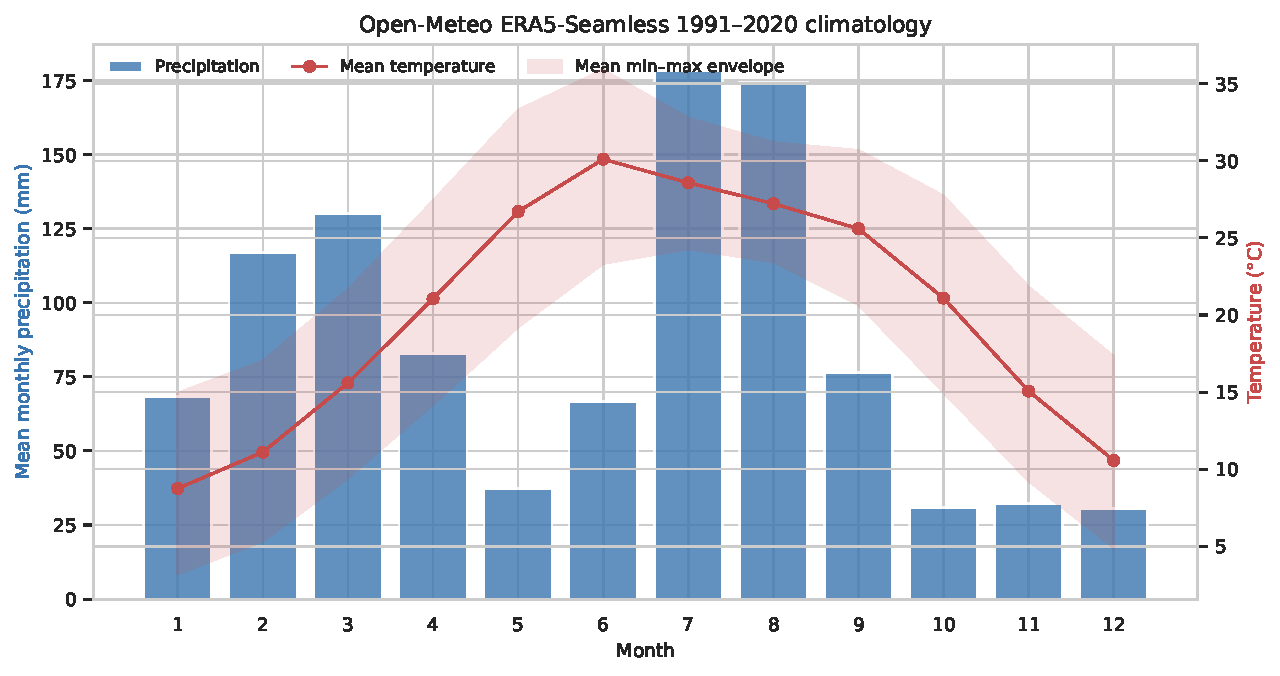
\includegraphics[width=\textwidth,height=.77\textheight,keepaspectratio]{figure_s03_climatology.pdf}\caption{Daily climatology of the regional four-cell average, 1991--2025, showing the post-monsoon window from which the Landsat composites are drawn.}\label{fig:s-clim}
\end{figure}
\begin{figure}[p]\centering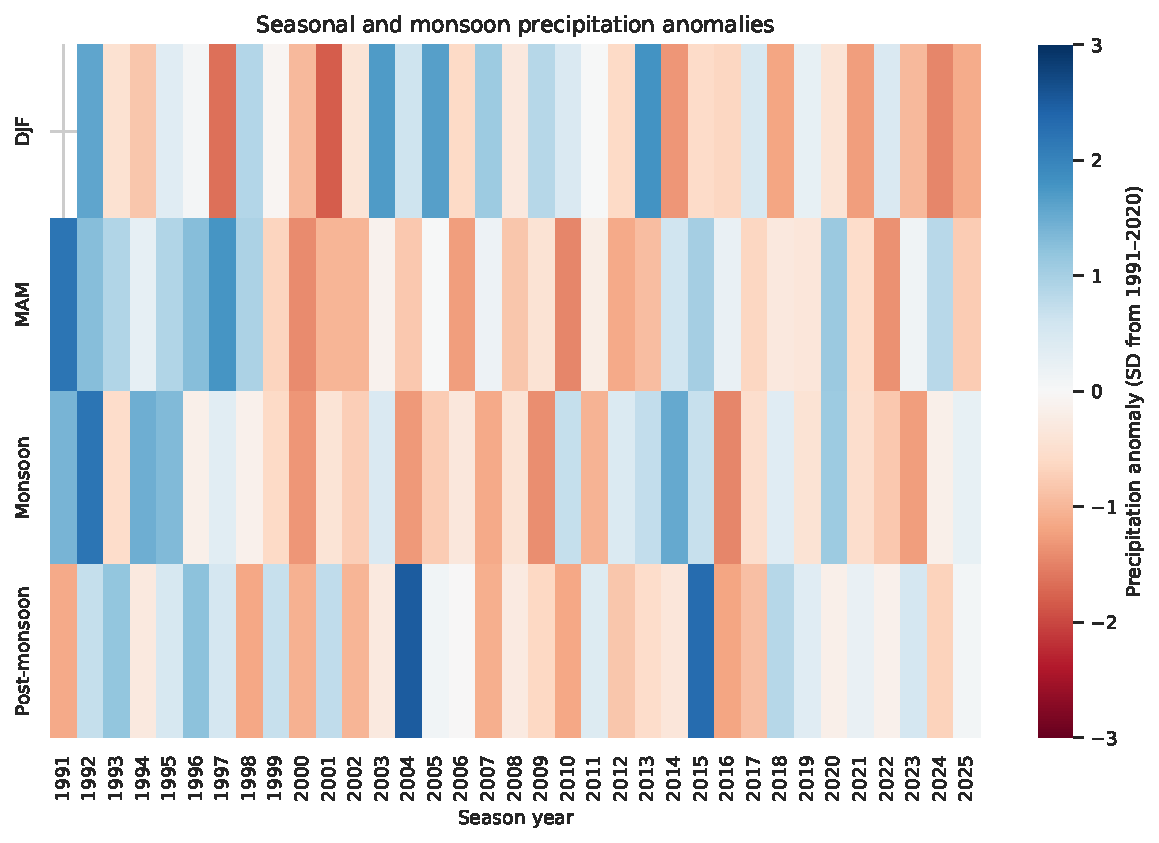
\includegraphics[width=\textwidth,height=.77\textheight,keepaspectratio]{figure_s04_seasonal_anomalies.pdf}\caption{Seasonal precipitation and temperature anomalies by year. Anomalies are relative to the 1991--2025 seasonal means of the same product.}\label{fig:s-anom}
\end{figure}
\begin{figure}[p]\centering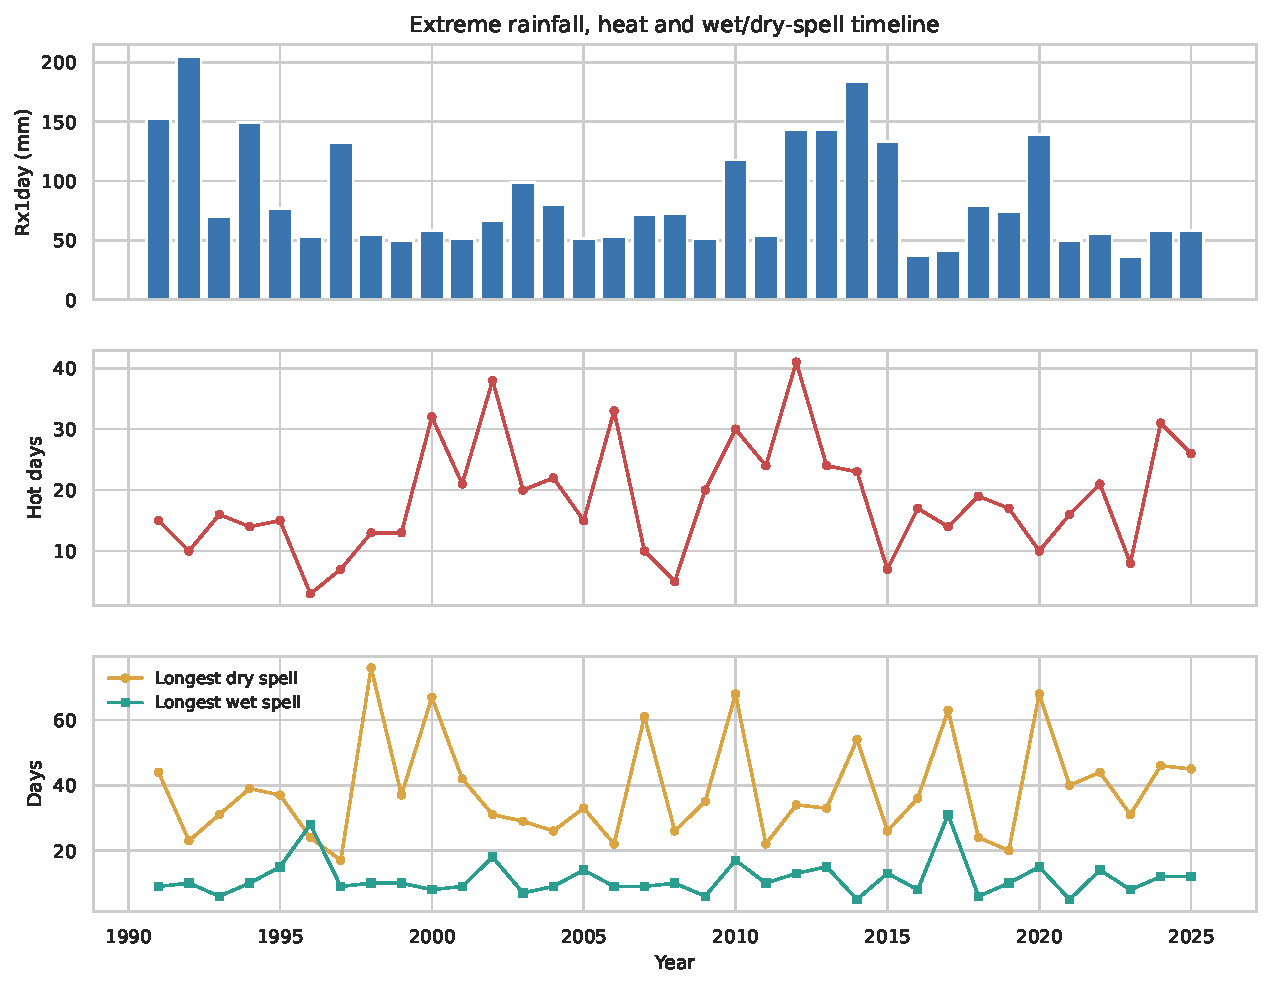
\includegraphics[width=\textwidth,height=.77\textheight,keepaspectratio]{figure_s05_extreme_timeline.pdf}\caption{Timeline of heavy-precipitation and heat days. Event thresholds are defined in Section~S6.}\label{fig:s-extreme}
\end{figure}
\begin{figure}[p]\centering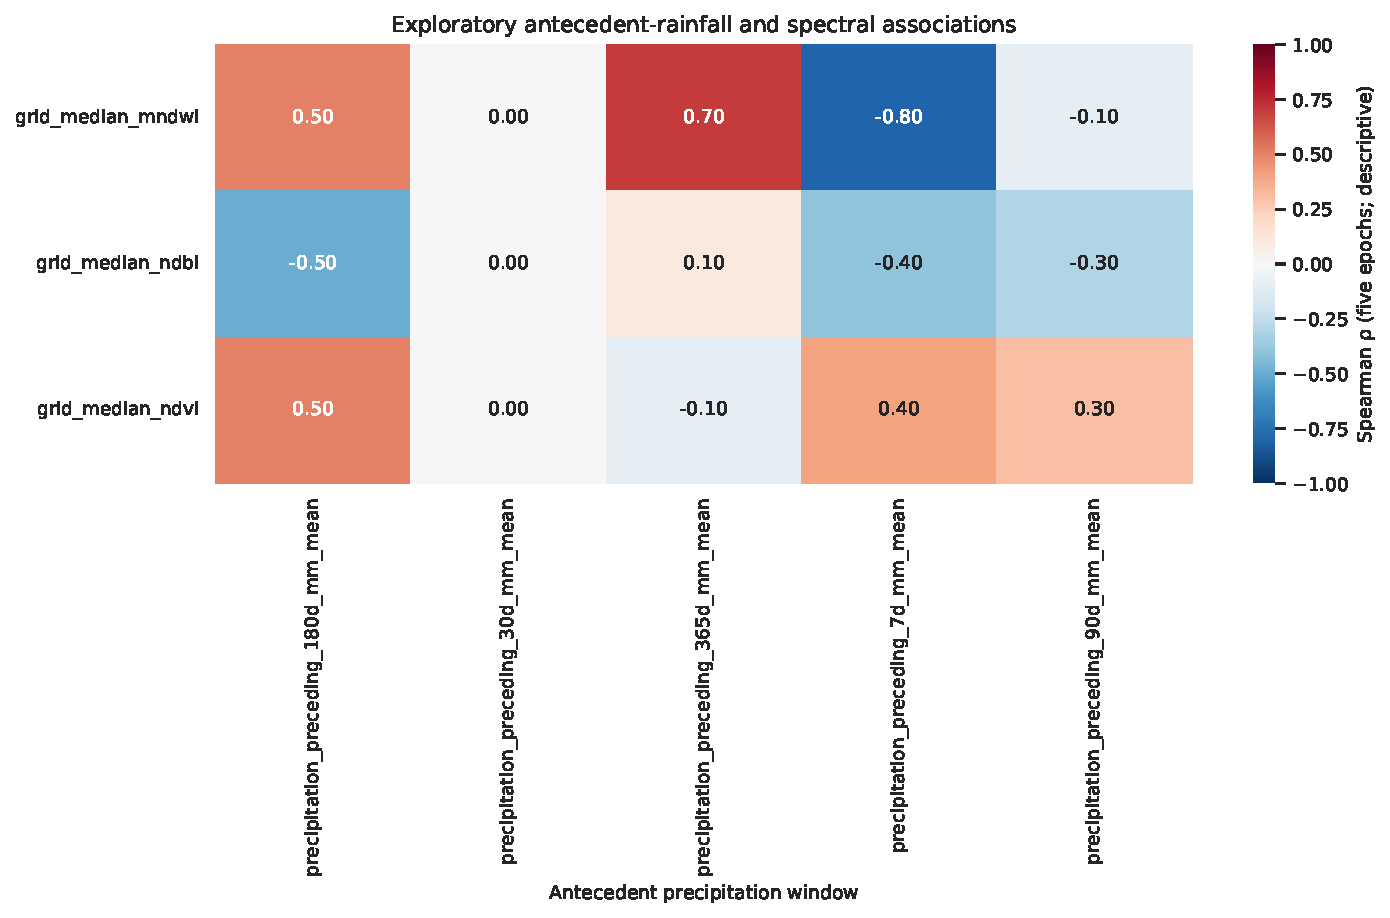
\includegraphics[width=\textwidth,height=.77\textheight,keepaspectratio]{figure_s06_weather_spectral_associations.pdf}\caption{Associations between antecedent weather windows and component spectral summaries. Five composite epochs provide only five temporal replicates, so these associations are underpowered and are reported as diagnostics, not findings.}\label{fig:s-assoc}
\end{figure}
\begin{figure}[p]\centering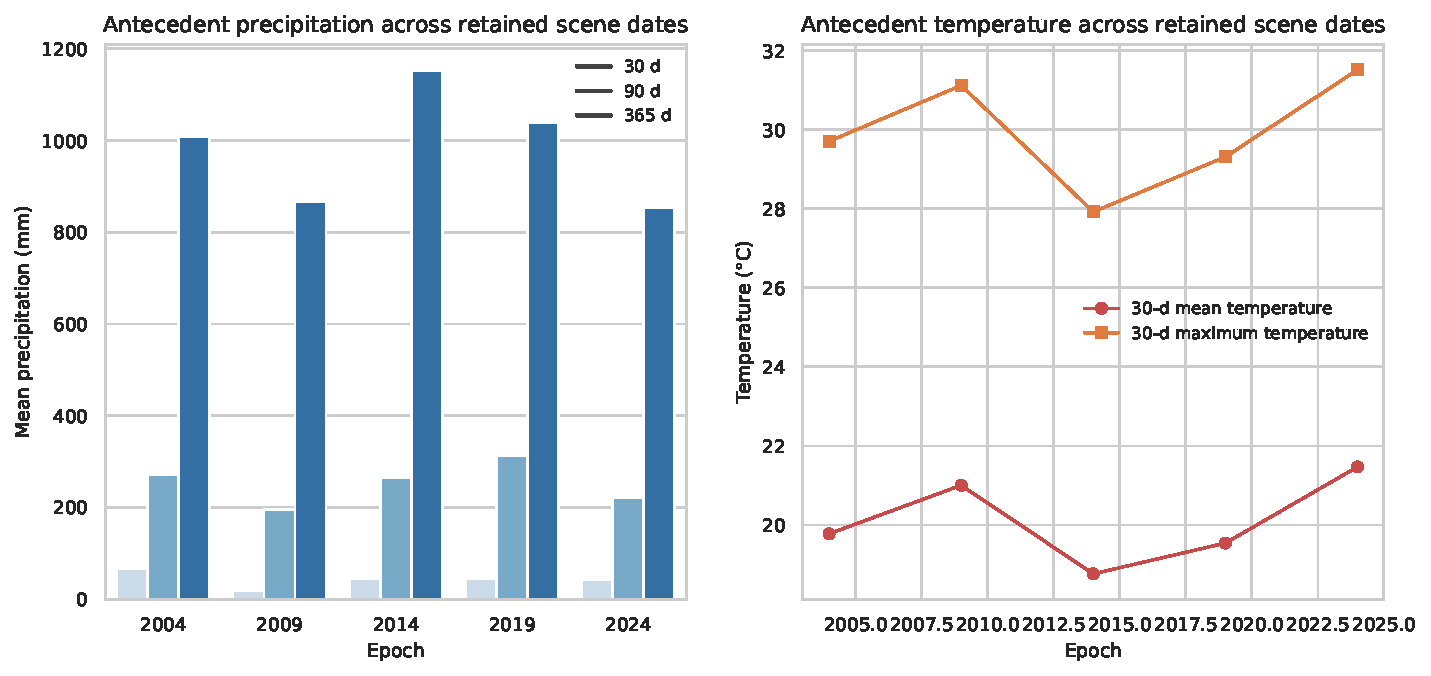
\includegraphics[width=\textwidth,height=.77\textheight,keepaspectratio]{figure_s07_epoch_specific_weather_forcing.pdf}\caption{Weather matched to the retained Landsat acquisition windows; contextual rather than causal.}\end{figure}
\begin{figure}[p]\centering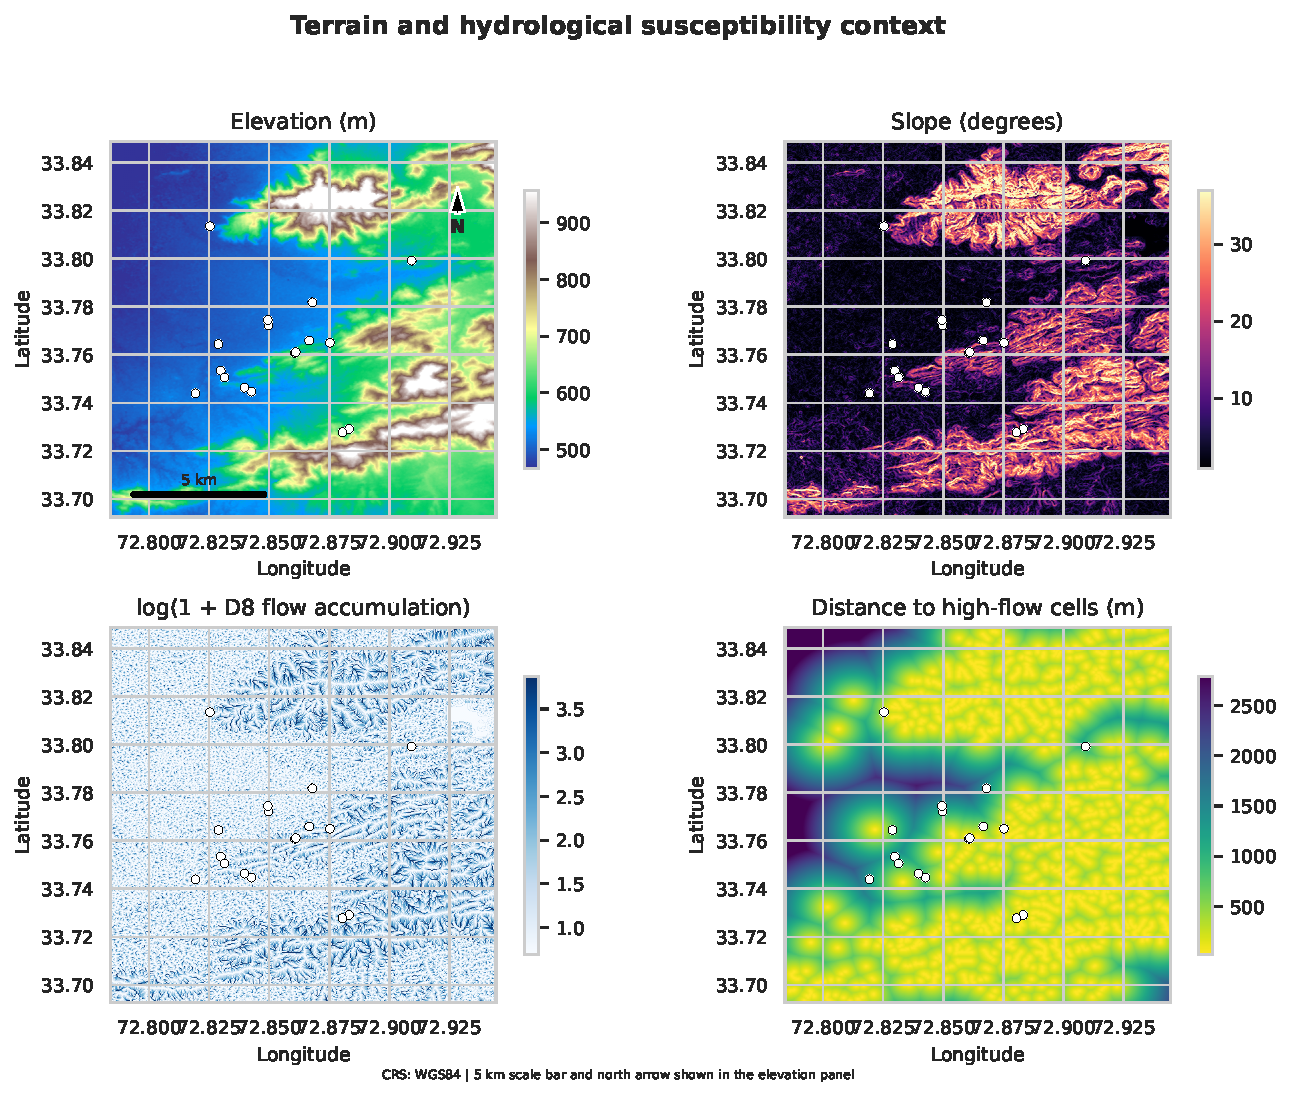
\includegraphics[width=\textwidth,height=.77\textheight,keepaspectratio]{figure_s08_terrain_hydrological_susceptibility.pdf}\caption{Elevation-derived terrain and drainage proxies. These do not constitute a hydraulic model.}\end{figure}
\begin{figure}[p]\centering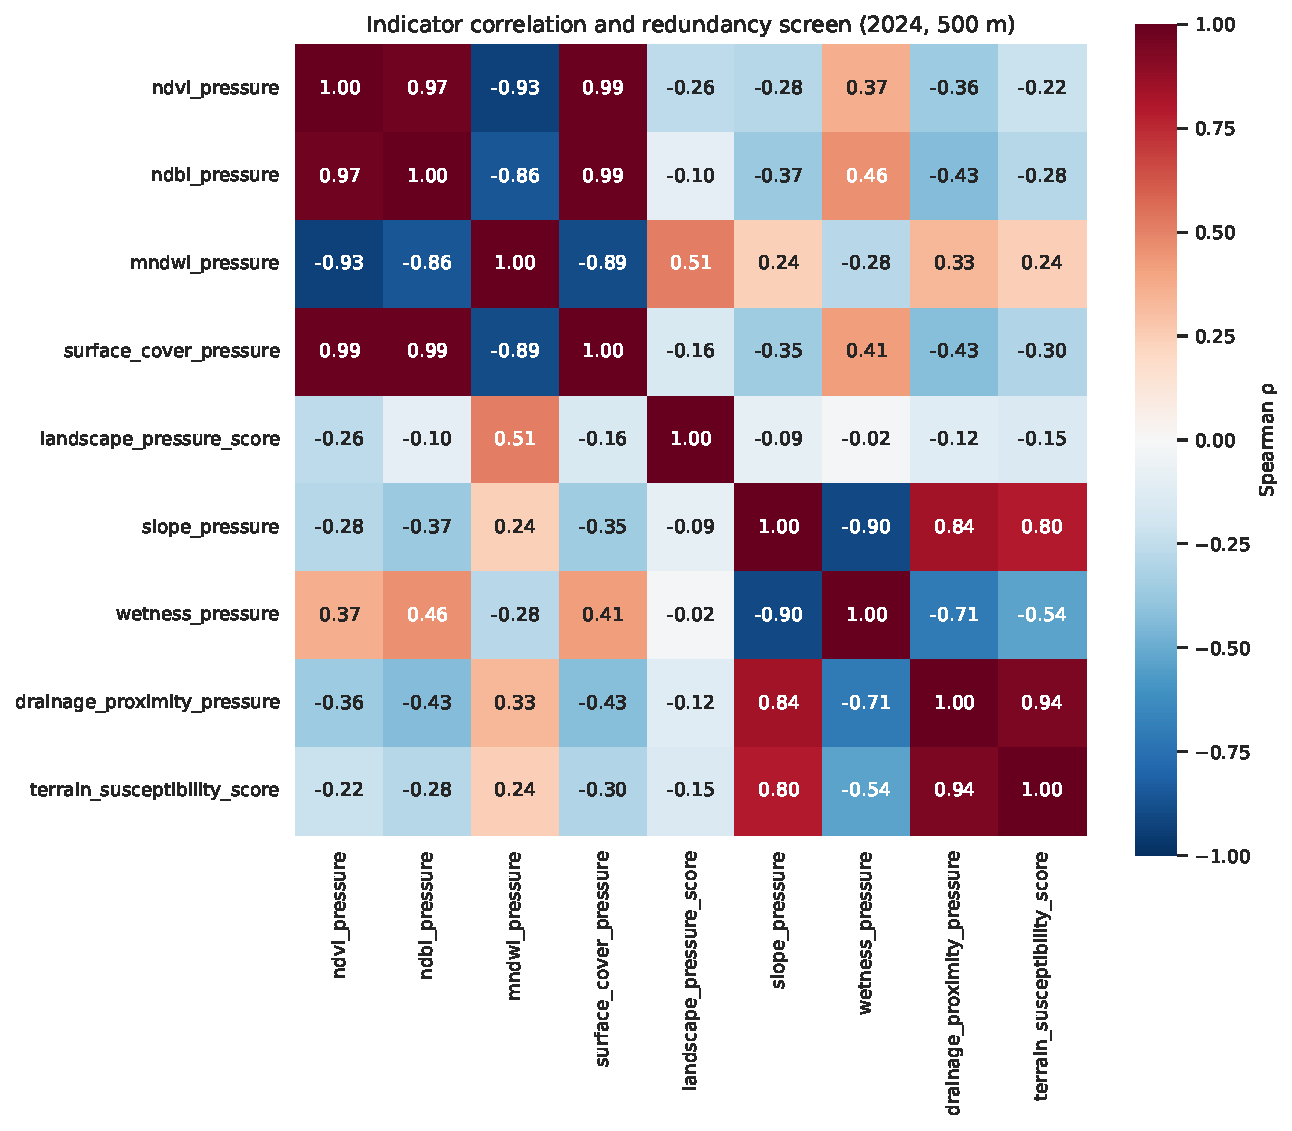
\includegraphics[width=\textwidth,height=.77\textheight,keepaspectratio]{figure_s09_indicator_redundancy.pdf}\caption{Dependence among component-level indicator ranks.}\end{figure}
\end{document}
